\chapter{Time Series}\label{time-series}

A time series is a sequence where a stochastic process is recorded over regular time intervals. Depending on the frequency, a time series can be of yearly (annual budget), quarterly (expenses), monthly (air traffic), weekly (sales qty), daily (weather), hourly (stocks price), minutes (inbound calls in a call canter) or even seconds wise (web traffic).

It is very important to learn how to analyze a time series because it is the preparatory step before you develop a forecast of the series. Besides, time series forecasting has enormous commercial significance because stuff that is important to a business like demand and sales, number of visitors to a website, stock price etc are essentially time series data. Time series analysis involves understanding various aspects about the inherent nature of the series so that you are better informed to create meaningful and accurate forecasts.

\section{Visualizing Time Series}\label{visualizing-time-series}

The data for a time series typically is stored in \texttt{.csv} files or other spreadsheet formats and contains two columns: the date and the measured value. Sometimes it may contains one or more related variables that are measured for the same time periods.

Clearly the best instrument to deal with time series is the \(\tt{pandas}\) package. In the following we are going to use an example data-set counting the total monthly scripts for pharmaceutical products fighting diabet, \href{https://raw.githubusercontent.com/matteosan1/finance_course/develop/libro/input_files/a10.csv}{a10.csv}.

\begin{ipython}
import pandas as pd

df = pd.read_csv('a10.csv', parse_dates=['date'], index_col='date')
print (df.head())
\end{ipython}
\begin{ioutput}
               value
date
1991-07-01  3.526591
1991-08-01  3.180891
1991-09-01  3.252221
1991-10-01  3.611003
1991-11-01  3.565869
\end{ioutput}
        
%\begin{codebox}[breakable, size=fbox, boxrule=1pt, pad at break*=1mm,colback=cellbackground, colframe=cellborder]
%\begin{Verbatim}[commandchars=\\\{\}]
%\PY{k+kn}{import} \PY{n+nn}{matplotlib} \PY{k}{as} \PY{n+nn}{mpl}
%\PY{k+kn}{import} \PY{n+nn}{matplotlib}\PY{n+nn}{.}\PY{n+nn}{pyplot} \PY{k}{as} \PY{n+nn}{plt}
%
%\PY{k}{def} \PY{n+nf}{plot\PYZus{}df}\PY{p}{(}\PY{n}{df}\PY{p}{,} \PY{n}{x}\PY{p}{,} \PY{n}{y}\PY{p}{,} \PY{n}{title}\PY{o}{=}\PY{l+s+s2}{\PYZdq{}}\PY{l+s+s2}{\PYZdq{}}\PY{p}{,} \PY{n}{xlabel}\PY{o}{=}\PY{l+s+s1}{\PYZsq{}}\PY{l+s+s1}{Date}\PY{l+s+s1}{\PYZsq{}}\PY{p}{,} \PY{n}{ylabel}\PY{o}{=}\PY{l+s+s1}{\PYZsq{}}\PY{l+s+s1}{Value}\PY{l+s+s1}{\PYZsq{}}\PY{p}{)}\PY{p}{:}
%    \PY{n}{plt}\PY{o}{.}\PY{n}{figure}\PY{p}{(}\PY{n}{figsize}\PY{o}{=}\PY{p}{(}\PY{l+m+mi}{10}\PY{p}{,}\PY{l+m+mi}{8}\PY{p}{)}\PY{p}{)}
%    \PY{n}{plt}\PY{o}{.}\PY{n}{plot}\PY{p}{(}\PY{n}{x}\PY{p}{,} \PY{n}{y}\PY{p}{,} \PY{n}{color}\PY{o}{=}\PY{l+s+s1}{\PYZsq{}}\PY{l+s+s1}{tab:red}\PY{l+s+s1}{\PYZsq{}}\PY{p}{)}
%    \PY{n}{plt}\PY{o}{.}\PY{n}{gca}\PY{p}{(}\PY{p}{)}\PY{o}{.}\PY{n}{set}\PY{p}{(}\PY{n}{title}\PY{o}{=}\PY{n}{title}\PY{p}{,} \PY{n}{xlabel}\PY{o}{=}\PY{n}{xlabel}\PY{p}{,} \PY{n}{ylabel}\PY{o}{=}\PY{n}{ylabel}\PY{p}{)}
%    \PY{n}{plt}\PY{o}{.}\PY{n}{show}\PY{p}{(}\PY{p}{)}
%
%\PY{n}{plot\PYZus{}df}\PY{p}{(}\PY{n}{df}\PY{p}{,} \PY{n}{x}\PY{o}{=}\PY{n}{df}\PY{o}{.}\PY{n}{index}\PY{p}{,} \PY{n}{y}\PY{o}{=}\PY{n}{df}\PY{o}{.}\PY{n}{value}\PY{p}{,} 
%        \PY{n}{title}\PY{o}{=}\PY{l+s+s1}{\PYZsq{}}\PY{l+s+s1}{Monthly anti\PYZhy{}diabetic drug sales in Australia from 1992 to 2008.}\PY{l+s+s1}{\PYZsq{}}\PY{p}{)}    
%\end{Verbatim}
%\end{codebox}

\begin{figure}[htb]
	\centering
	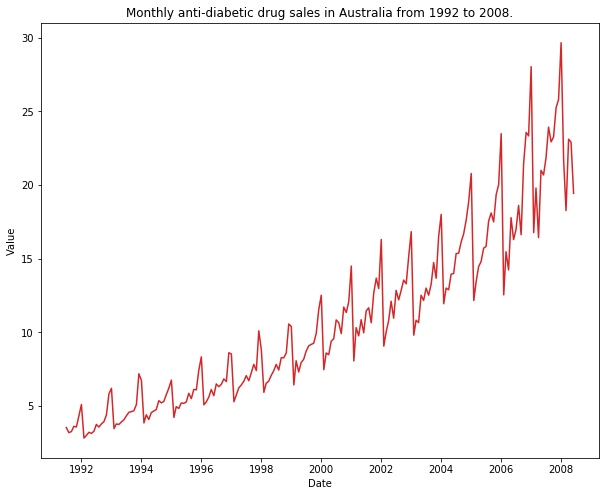
\includegraphics[width=0.7\linewidth]{figures/drug_dataset.png}
	\caption{Time series counting the total monthly scripts for pharmaceutical anti-diabetic products.}
	\label{fig:drug_dataset}
\end{figure}
    
Since its a monthly time series and follows a certain repetitive pattern
every year, you can plot each year as a separate line in the same plot.
This lets you compare the year wise patterns side-by-side.

\begin{ipython}
import numpy as np

df.reset_index(inplace=True)
df['year'] = [d.year for d in df.date]
df['month'] = [d.strftime('%b') for d in df.date]
years = df['year'].unique()
\end{ipython}

\begin{figure}[htb]
	\centering
	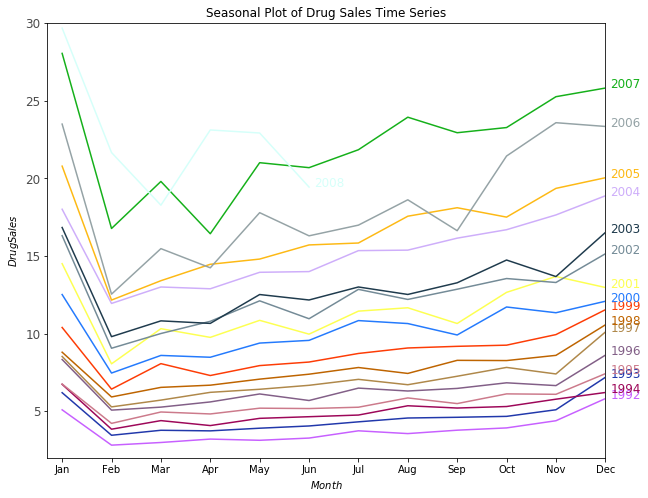
\includegraphics[width=0.7\linewidth]{figures/yearly_drug_dataset.png}
	\caption{Yearly time series counting the total monthly scripts for pharmaceutical anti-diabetic products.}
	\label{fig:yearly_drug_dataset}
\end{figure}
    
There is a steep fall in drug sales every February, rising again in
March, falling again in April and so on. Clearly, the pattern repeats
within a given year, every year.

\section{Patterns in a time series}\label{patterns-in-a-time-series}

So far, we have seen the similarities to identify the pattern. Now, how
to find out any deviations from the usual pattern? Any time series may
be split into the following components

\begin{itemize}
\tightlist
\item
  base level;
\item
  trend: is observed when there is an increasing or decreasing slope
  observed in the time series;
\item
  seasonality: is observed when there is a distinct repeated pattern
  observed between regular intervals due to seasonal factors. It could
  be because of the month of the year, the day of the month, weekdays or
  even time of the day;
\item
  error.
\end{itemize}

It is not mandatory that all time series must have a trend and/or
seasonality. A time series may not have a distinct trend but have a
seasonality. The opposite can also be true. So, a time series may be
imagined as a combination of the trend, seasonality and the error terms.

\begin{figure}[htb]
	\centering
	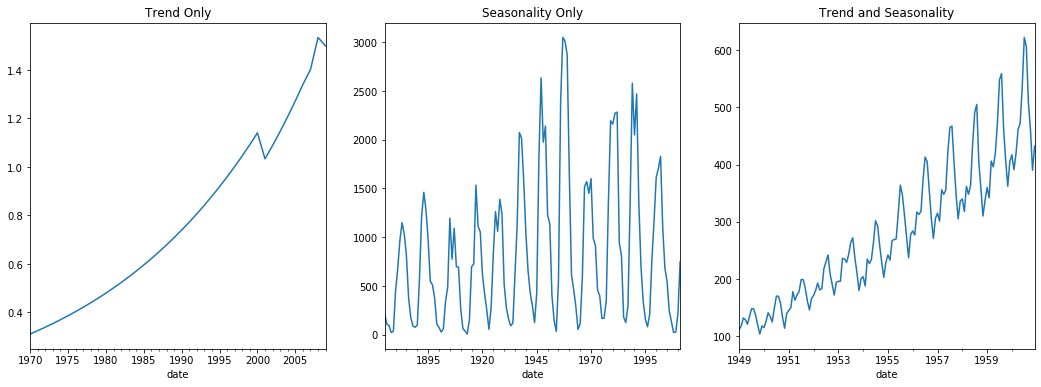
\includegraphics[width=0.9\linewidth]{figures/time_series_patterns.png}
	\caption{Examples of time series with patterns: trend only (left), seasonality only (center), trend and seasonality (right).}
	\label{fig:time_series_patterns}
\end{figure}
    
Another aspect to consider is the cyclic behaviour. It happens when the
rise and fall pattern in the series does not happen in fixed
calendar-based intervals. Care should be taken to not confuse `cyclic'
effect with `seasonal' effect. If the patterns are not of fixed calendar
based frequencies, then it is cyclic. Because, unlike the seasonality,
cyclic effects are typically influenced by the business and other
socio-economic factors.

\section{Time Series Modelling}\label{time-series-modelling}

In this Section we are going to describe two simple models to describe
time series.

\subsection{Autoregression (AR)}\label{autoregression-ar}

A regression model, such as linear regression, models an output value
based on a linear combination of input values (see Section~\ref{sec:capm}). For
example:

\begin{equation}
\hat{y} = \hat{\alpha} + \hat{\beta}X
\end{equation} 
where \(\hat{y}\) is the prediction, \(\hat{\alpha}\) and \(\hat{\beta}\) are coefficients found
by optimizing the model on training data, and \(X\) is an input value.

This technique can be used on time series too where input variables are
taken as observations at previous time steps, called
\emph{lag variables}.

For example, we can express the value for the next time step \(t\) given
the observations at the last two time steps (\(t-1\) and \(t-2\)). As a
regression model, this would look as follows:

\begin{equation}
Y_{t} = \phi_0 + \phi_1Y_{t-1} + \phi_2Y_{t-2}
\end{equation}

Because the regression model uses data from the same input variable at
previous time steps, it is referred to as an \emph{autoregression}
(regression of itself). The autoregression (AR) model describes the next
step in the sequence as a linear function of the observations at prior
time steps. A pure Auto Regressive (AR only) model is one where \(Y_t\)
depends only on its own lags. That is, \(Y_t\) is a function of the
`lags of \(Y_t\)'

\begin{equation}
Y_t = \phi_0 + \phi_1 Y_{t-1} + \phi_2 Y_{t-2} + \ldots + \phi_p Y_{t-p} + \ldots + \epsilon_t
\label{eq:ar}
\end{equation}
where, \(Y_{t-1}\) is the lag-1 of the series, \(\phi_1\) is the
coefficient of lag-1 that the model estimates and \(\phi_0\) is the
intercept term, also estimated by the model. \(\epsilon_t\) is the error
associated to the estimate of the time series at time \(t\) (since it 
is anyway a stochastic process) and it is
usually normally distributed (\(\mathcal{N}(0, \sigma^2)\)), also called
\emph{white noise process}.

The number of lags used in the model is called \emph{order} (\(p\)) 
and the  notation involves specifying this value as 
a parameter to the function, AR(\(p\)). For example,
AR(1) is a first-order autoregression model.

This kind of model can be easily coded in \(\tt{python}\). Figure~\ref{fig:ar2_example} shows an example of AR(2) time series.

\begin{ipython}
def AR(x, phi):
    val = phi[0]
    for i, b in enumerate(phi[1:]):
        val += b * x[-(i+1)]
    return val + np.random.normal()

phi = [0, 0.5, -0.7]
x = [0, 0]
for _ in range(100):
    x.append(AR(x, phi))
\end{ipython}

\begin{figure}[htb]
	\centering
	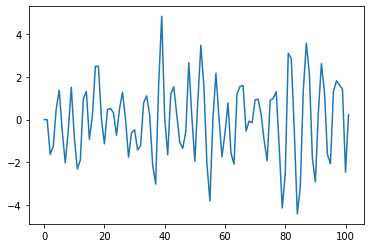
\includegraphics[width=0.7\linewidth]{figures/ar2.png}
	\caption{Examples of AR(2) time series produced by the code shown in this Section.}
	\label{fig:ar2_example}
\end{figure}
   
\subsection{Moving Average (MA)}\label{moving-average-ma}

The moving average (MA) is another common approach for modeling univariate time series. It models the next step in the sequence as a linear function of the residual errors from a mean process at prior time steps

\begin{equation}
Y_t = \mu + \theta_1 \epsilon_{t-1} + \theta_2 \epsilon_{t-2} + \ldots + \theta_q \epsilon_{t-q} + \epsilon_t
\end{equation}
where \(\mu\) is the mean of the series, the \(\theta_1, \ldots, \theta_q\) are the parameters of the model and the \(\epsilon_t, \epsilon_{t−1},..., \epsilon_{t−q}\) are the error terms.

Thus, a moving-average model is conceptually a linear regression of the current value of the series against current and previous (observed) error terms. Those terms at each point are assumed to be mutually independent and to come from the same distribution, typically a normal distribution, with zero mean and constant variance. Beware that a moving average model is different from calculating the moving average of the time series.

The error terms refer to the errors of the autoregressive models of the respective lags. The errors \(\epsilon_t\) and \(\epsilon_{t-1}\) are determined from the following equations:

\begin{equation}
\begin{gathered}
Y_t = \phi_1 Y_{t-1} + \phi_2 Y_{t-2} + \ldots + \phi_0 Y_{0} + \epsilon_t
Y_{t-1} = \phi_2 Y_{t-2} + \phi_3 Y_{t-3} + \ldots + \phi_0 Y_{0} + \epsilon_{t-1}
\end{gathered}
\end{equation}

The notation for the model involves specifying the order of the model $q$ as a parameter as in MA($q$). For example, MA(1) is a
first-order moving average model. 

\section{Stationary and Non-Stationary Time Series}
\label{stationary-and-non-stationary-time-series}

A stationary series is one where the values of the series is not a function of time. That is, the statistical properties of the series like mean, variance and autocorrelation are constant over time. A stationary time series is lacking of seasonal effects too.

%\begin{codebox}[breakable, size=fbox, boxrule=1pt, pad at break*=1mm,colback=cellbackground, colframe=cellborder]
%\begin{Verbatim}[commandchars=\\\{\}]
%\PY{c+c1}{\PYZsh{} plot of stationary and not stationary series}
%\PY{k}{def} \PY{n+nf}{f}\PY{p}{(}\PY{n}{x}\PY{p}{,} \PY{n}{phi}\PY{p}{)}\PY{p}{:}
%    \PY{k}{return} \PY{n}{phi}\PY{o}{*}\PY{n}{x} \PY{o}{+} \PY{n}{np}\PY{o}{.}\PY{n}{random}\PY{o}{.}\PY{n}{normal}\PY{p}{(}\PY{p}{)}
%
%\PY{n}{phi} \PY{o}{=} \PY{l+m+mf}{0.5}
%\PY{n}{x} \PY{o}{=} \PY{p}{[}\PY{n}{f}\PY{p}{(}\PY{l+m+mi}{1}\PY{p}{,}\PY{n}{phi}\PY{p}{)}\PY{p}{]}
%\PY{k}{for} \PY{n}{\PYZus{}} \PY{o+ow}{in} \PY{n+nb}{range}\PY{p}{(}\PY{l+m+mi}{500}\PY{p}{)}\PY{p}{:}
%    \PY{n}{x}\PY{o}{.}\PY{n}{append}\PY{p}{(}\PY{n}{f}\PY{p}{(}\PY{n}{x}\PY{p}{[}\PY{o}{\PYZhy{}}\PY{l+m+mi}{1}\PY{p}{]}\PY{p}{,} \PY{n}{phi}\PY{p}{)}\PY{p}{)}
%
%\PY{n}{phi} \PY{o}{=} \PY{l+m+mf}{1.051}
%\PY{n}{x1} \PY{o}{=} \PY{p}{[}\PY{n}{f}\PY{p}{(}\PY{l+m+mi}{1}\PY{p}{,}\PY{n}{phi}\PY{p}{)}\PY{p}{]}
%\PY{k}{for} \PY{n}{\PYZus{}} \PY{o+ow}{in} \PY{n+nb}{range}\PY{p}{(}\PY{l+m+mi}{50}\PY{p}{)}\PY{p}{:}
%    \PY{n}{x1}\PY{o}{.}\PY{n}{append}\PY{p}{(}\PY{n}{f}\PY{p}{(}\PY{n}{x1}\PY{p}{[}\PY{o}{\PYZhy{}}\PY{l+m+mi}{1}\PY{p}{]}\PY{p}{,} \PY{n}{phi}\PY{p}{)}\PY{p}{)}
%    
%\PY{n}{plt}\PY{o}{.}\PY{n}{figure}\PY{p}{(}\PY{n}{figsize}\PY{o}{=}\PY{p}{(}\PY{l+m+mi}{12}\PY{p}{,} \PY{l+m+mi}{6}\PY{p}{)}\PY{p}{)}
%\PY{n}{plt}\PY{o}{.}\PY{n}{subplot}\PY{p}{(}\PY{l+m+mi}{1}\PY{p}{,} \PY{l+m+mi}{2}\PY{p}{,} \PY{l+m+mi}{1}\PY{p}{)}
%\PY{n}{plt}\PY{o}{.}\PY{n}{title}\PY{p}{(}\PY{l+s+s2}{\PYZdq{}}\PY{l+s+s2}{Stationary Series}\PY{l+s+s2}{\PYZdq{}}\PY{p}{)}
%\PY{n}{plt}\PY{o}{.}\PY{n}{plot}\PY{p}{(}\PY{n}{x}\PY{p}{)}
%\PY{n}{plt}\PY{o}{.}\PY{n}{subplot}\PY{p}{(}\PY{l+m+mi}{1}\PY{p}{,} \PY{l+m+mi}{2}\PY{p}{,} \PY{l+m+mi}{2}\PY{p}{)}
%\PY{n}{plt}\PY{o}{.}\PY{n}{title}\PY{p}{(}\PY{l+s+s2}{\PYZdq{}}\PY{l+s+s2}{Non Stationary Series}\PY{l+s+s2}{\PYZdq{}}\PY{p}{)}
%\PY{n}{plt}\PY{o}{.}\PY{n}{plot}\PY{p}{(}\PY{n}{x1}\PY{p}{)}
%\PY{n}{plt}\PY{o}{.}\PY{n}{show}\PY{p}{(}\PY{p}{)}
%\end{Verbatim}
%\end{codebox}

\begin{figure}[htb]
	\centering
	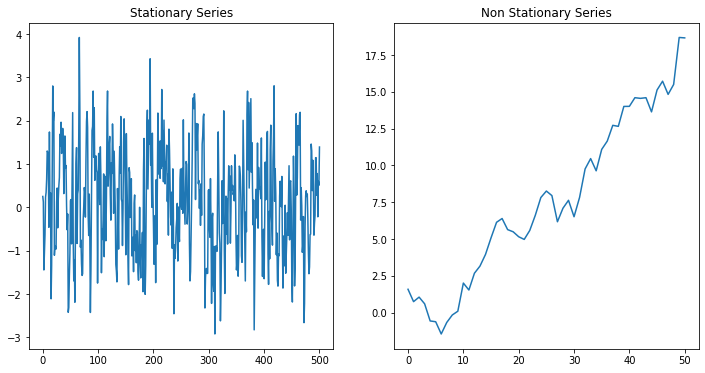
\includegraphics[width=0.7\linewidth]{figures/stationary_and_non_stationary.png}
	\caption{Example of a stationary (left) and non-stationary (right) time series.}
	\label{fig:stationary_non_stationary}
\end{figure}
        
MA series are always stationary since both mean and variance are constant in time. Indeed for the mean we have that

\begin{equation}
\mathbb{E}(\textrm{MA}(q)) = \mu + \sum_{q}\theta_{t-q}\mathbb{E}(\epsilon_{t-q}) = \mu
\end{equation}
while for the variance we have to remember that the \(\epsilon_t\) are
all independent identical distributed variable with constant variance so (the variance of the sum of independent Gaussian is the sum of the single variances)
\begin{equation}
\textrm{var(MA(}q)) = \sigma^2 \sum_{q}\theta_{t-q}
\end{equation}

Contrary AR series are not always stationary. Consider for example an AR(1) process which is given by:

\begin{equation} 
Y_t = c + \phi_1 Y_{t−1} + \epsilon_t
\end{equation}
where \(\epsilon_{t}\) is a
white noise process with zero mean and constant variance \(\sigma_{\epsilon}^2\). If we recurse back in time a couple of time we
have

\begin{equation}
\begin{aligned}
Y_t &= c + \phi_1 Y_{t−1} + \epsilon_t = c + c\phi_1 + \phi_1^2 Y_{t-2} + \epsilon_t + \phi_1 \epsilon_{t-1} = \\
&= c + c\phi_1 + c\phi_1^2 + \phi_1^3 Y_{t-3} + \epsilon_t + \phi_1 \epsilon_{t-1} + \phi_1^2 \epsilon_{t-2}
\end{aligned}
\end{equation}
Now imagine to repeat the process \(j\) times we have

\begin{equation}
Y_t = c[\sum_{s=0}^j \phi_1^s Y_{t−1}] + \phi_1^{j+1} Y_{t-j-1} + \sum_{s=0}^j \phi_1^s \epsilon_{t-s}
\end{equation}

In the limit $j\rightarrow\infty$ (infinite series), the first sum becomes a \emph{geometric progressions} which converge to

\begin{equation}
c[\sum_{s=0}^j \phi_1^s Y_{t−1}] \underset{j\rightarrow\infty}{=} \cfrac{c}{1-\phi_1}
\end{equation}

The second term tends to 0 if \(|\phi_1| < 1\) otherwise it is infinite. So the expectation becomes:

\begin{equation}
\mathbb{E}(Y_t) =
\begin{cases}
\cfrac{c}{1-\phi_1} + \mathbb{E}(\sum_{s=0}^{\infty} \phi_1^s \epsilon_{t-s})\quad (\textrm{with } |\phi_1| < 1), \\
\infty + \mathbb{E}(\sum_{s=0}^{\infty} \phi_1^s \epsilon_{t-s})\quad (\textrm{with } |\phi_1| >= 1)
\end{cases}
\end{equation}
the last term is zero in the first case since \(\epsilon_t\) is a zero mean distributed random variable. With similar calculation we can find that the variance is given by

\begin{equation}
\textrm{var}(Y_t) = \mathbb{E}(Y_t^2) − \frac{c^2}{(1-\phi_1)^2} = \frac{\sigma_{\epsilon}^2}{1-\phi_1^2}
\end{equation}
where \(\sigma_{\epsilon}\) is the standard deviation of the white noise process. Hence we can conclude that the series is stationary if \(|\phi_1| < 1\).

\subsection{White Noise}\label{white-noise}

White noise is particular example of stationary series. Its mean and variance does not change over time, the peculiarity is that the mean is constant at 0.

If you consider the sound signals in an FM radio as a time series, the blank sound you hear between the channels is white noise.
Mathematically, a sequence of completely random numbers with mean zero is a white noise.

\begin{figure}[htb]
	\centering
	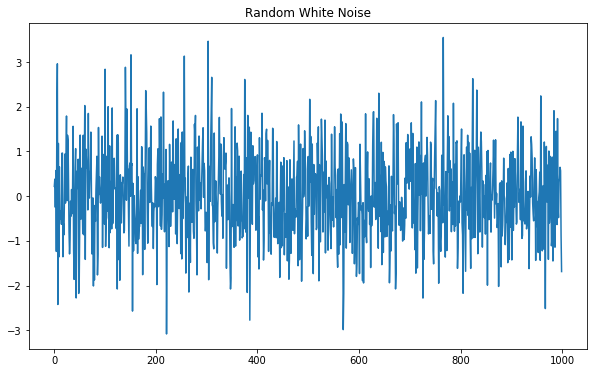
\includegraphics[width=0.7\linewidth]{figures/white_noise.png}
	\caption{White noise distribution example.}
	\label{fig:white_noise}
\end{figure}

\subsection{Making a Non Stationary Series Stationary}
\label{making-a-non-stationary-series-stationary}

It is possible to make nearly any time series stationary by applying a suitable transformation. This is useful since most statistical forecasting methods are designed to work on a stationary time series.

You can make series stationary by:

\begin{itemize}
\tightlist
\item
  differencing the series (once or more times);
\item
  take the log of the series;
\item
  take the nth root of the series;
\item
  combination of the above.
\end{itemize}

The most common and convenient method to stationarize the series (and the only one we are going to look at) is by differencing it until becomes approximately stationary.

If \(Y_t\) is the value at time \(t\), then the first difference is \(Y = Y_t - Y_{t-1}\). In simpler terms, it means
nothing but subtracting the next value by the current value. If the first difference doesn't make a series stationary, you can go for the second differencing. And so on.

For example, consider the following series: $\{1, 5, 2, 12, 20\}$.
First differencing gives: $\{5-1, 2-5, 12-2, 20-12\} = \{4, -3, 10, 8\}$,
second differencing gives: $\{-3-4, -10-3, 8-10\} = \{-7, -13, -2\}$.

%SPOSTARE There are various reasons why we have to make a non-stationary
%series stationary before forecasting:
%
%\begin{itemize}
%\tightlist
%\item
%  forecasting a stationary series is relatively easy and the forecasts
%  are more reliable;
%\item
%  autoregressive forecasting models (AR models) are essentially linear
%  regression models that utilize the lag(s) of the series itself as
%  predictors. We know that linear regression works best if the
%  predictors (\(X\) variables) are not correlated against each other.
%  So, stationarizing the series solves this problem since it removes any
%  persistent autocorrelation, thereby making the predictors(lags of the
%  series) in the forecasting models nearly independent.
%\end{itemize}
%
%\begin{codebox}[breakable, size=fbox, boxrule=1pt, pad at break*=1mm,colback=cellbackground, colframe=cellborder]
%\begin{Verbatim}[commandchars=\\\{\}]
%\PY{n}{y} \PY{o}{=} \PY{p}{[}\PY{p}{]}
%\PY{k}{for} \PY{n}{i} \PY{o+ow}{in} \PY{n+nb}{range}\PY{p}{(}\PY{l+m+mi}{2}\PY{p}{,} \PY{n+nb}{len}\PY{p}{(}\PY{n}{x1}\PY{p}{)}\PY{p}{)}\PY{p}{:}
%    \PY{n}{y}\PY{o}{.}\PY{n}{append}\PY{p}{(}\PY{n}{x1}\PY{p}{[}\PY{n}{i}\PY{p}{]} \PY{o}{\PYZhy{}} \PY{n}{x1}\PY{p}{[}\PY{n}{i}\PY{o}{\PYZhy{}}\PY{l+m+mi}{1}\PY{p}{]}\PY{p}{)}
%
%\PY{n}{y1} \PY{o}{=} \PY{p}{[}\PY{p}{]}
%\PY{k}{for} \PY{n}{i} \PY{o+ow}{in} \PY{n+nb}{range}\PY{p}{(}\PY{l+m+mi}{1}\PY{p}{,} \PY{n+nb}{len}\PY{p}{(}\PY{n}{y}\PY{p}{)}\PY{p}{)}\PY{p}{:}
%    \PY{n}{y1}\PY{o}{.}\PY{n}{append}\PY{p}{(}\PY{n}{y}\PY{p}{[}\PY{n}{i}\PY{p}{]} \PY{o}{\PYZhy{}} \PY{n}{y}\PY{p}{[}\PY{n}{i}\PY{o}{\PYZhy{}}\PY{l+m+mi}{1}\PY{p}{]}\PY{p}{)}
%
%\PY{n}{plt}\PY{o}{.}\PY{n}{figure}\PY{p}{(}\PY{n}{figsize}\PY{o}{=}\PY{p}{(}\PY{l+m+mi}{12}\PY{p}{,} \PY{l+m+mi}{6}\PY{p}{)}\PY{p}{)}
%\PY{n}{plt}\PY{o}{.}\PY{n}{subplot}\PY{p}{(}\PY{l+m+mi}{1}\PY{p}{,}\PY{l+m+mi}{2}\PY{p}{,}\PY{l+m+mi}{1}\PY{p}{)}
%\PY{n}{plt}\PY{o}{.}\PY{n}{title}\PY{p}{(}\PY{l+s+s2}{\PYZdq{}}\PY{l+s+s2}{First difference}\PY{l+s+s2}{\PYZdq{}}\PY{p}{)}
%\PY{n}{plt}\PY{o}{.}\PY{n}{plot}\PY{p}{(}\PY{n}{y}\PY{p}{)}
%\PY{n}{plt}\PY{o}{.}\PY{n}{ylim}\PY{p}{(}\PY{o}{\PYZhy{}}\PY{l+m+mi}{4}\PY{p}{,} \PY{l+m+mi}{4}\PY{p}{)}
%\PY{n}{plt}\PY{o}{.}\PY{n}{grid}\PY{p}{(}\PY{k+kc}{True}\PY{p}{)}
%\PY{n}{plt}\PY{o}{.}\PY{n}{subplot}\PY{p}{(}\PY{l+m+mi}{1}\PY{p}{,}\PY{l+m+mi}{2}\PY{p}{,}\PY{l+m+mi}{2}\PY{p}{)}
%\PY{n}{plt}\PY{o}{.}\PY{n}{title}\PY{p}{(}\PY{l+s+s2}{\PYZdq{}}\PY{l+s+s2}{Second difference}\PY{l+s+s2}{\PYZdq{}}\PY{p}{)}
%\PY{n}{plt}\PY{o}{.}\PY{n}{plot}\PY{p}{(}\PY{n}{y1}\PY{p}{)}
%\PY{n}{plt}\PY{o}{.}\PY{n}{ylim}\PY{p}{(}\PY{o}{\PYZhy{}}\PY{l+m+mi}{4}\PY{p}{,} \PY{l+m+mi}{4}\PY{p}{)}
%\PY{n}{plt}\PY{o}{.}\PY{n}{grid}\PY{p}{(}\PY{k+kc}{True}\PY{p}{)}
%\PY{n}{plt}\PY{o}{.}\PY{n}{show}\PY{p}{(}\PY{p}{)}
%\end{Verbatim}
%\end{codebox}

\begin{figure}[htb]
	\centering
	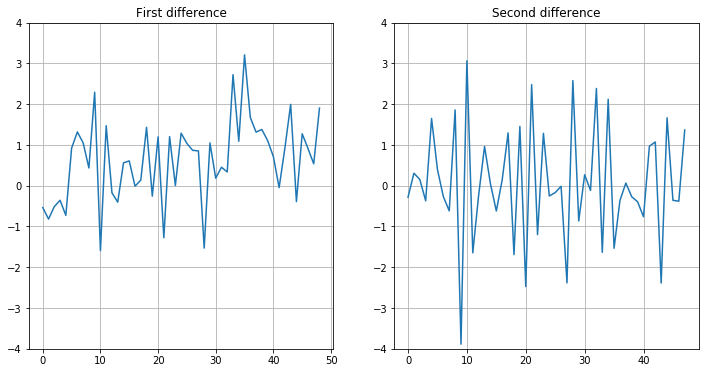
\includegraphics[width=0.7\linewidth]{figures/first_second_differencing.png}
	\caption{Example of first and second differencing of the non-stationary time series shown in Fig.~\ref{fig:stationary_non_stationary} (right).}
	\label{fig:1st_2nd_differencing}
\end{figure}
    
\subsection{Testing Stationarity}\label{testing-stationarity}

The stationarity of a series sometimes can be established by simply looking at its plot. Another method could be to split the series into 2 or more contiguous parts and computing the summary statistics like the mean and variance. If they are quite different then the series is not likely to be stationary.

Both these two techniques are not rigorous anyway, so a quantitative method to determine if a given series is stationary or not is needed. This can be done using statistical tests called \emph{unit root tests}. There are multiple implementations of such tests like:

\begin{itemize}
\tightlist
\item
  Augmented Dickey Fuller test (ADF Test)
\item
  Kwiatkowski-Phillips-Schmidt-Shin -- KPSS test (trend stationary)
\item
  Philips Perron test (PP Test)
\end{itemize}

In the next Section we will focus on the ADF test, but before we discuss briefly hypothesis testing in general.

\subsection{Hypothesis Testing}\label{hypothesis-testing}

All the tests mentioned above are statistical significance test. That means, there is a hypothesis testing involved with a null and an alternate hypothesis and as a result a test statistic is computed and the corresponding p-values get reported. It is from those (test statistic and the p-value) that an inference as to whether a given series is stationary or not can be made.

Let's first describe hypothesis testing in general starting with a simple example: imagine that you and a friend of yours play
a game. If a coin lands on heads, you win, if it lands on tails he wins.

Let's say the first two coin tosses landed on tails, meaning your friend won twice. Should you be worried that he's using a rigged coin ? Well, the probability of the coin landing on tails two times in a row is 25\% ($0.5\cdot 0.5$) which is not unlikely. 

What if the coin landed on tails six times in a row ? The probability of that occurring is approximately 1.56\% (\(0.5^6\)), which is highly unlikely. At this point, it would be fair to assume that the coin is rigged. Typically, one would set a threshold to determine if an event occurred by chance or not (this threshold is usually referred to as \(\alpha\))

To better understand hypothesis testing, let's describe some terminology:

\begin{itemize}
\tightlist
\item
  null hypothesis: the hypothesis that there is no significant difference between specified samples, any observed difference being   due to sampling or experimental error. In our example is that the coin is a fair coin and that the observations are purely from chance; 
\item
  alternative hypothesis: the hypothesis that sample observations are influenced by some non-random cause. The alternative hypothesis would then be that the coin is not fair, and thus, the observations did not happen by chance;
\item
  p-value: the probability of obtaining the observed results of a test, assuming that the null hypothesis is correct (i.e. a smaller p-value means that there is stronger evidence in favor of the alternative hypothesis). The p-value in the scenario of flipping tails 2 times in a row is 25\% and 6 times in a row is 1.56\%;
\item
  \(\alpha\): the significance level; the probability of rejecting the null hypothesis when it is true (also known as type 1 error). The \(\alpha\) or level of significance usually is set to 5\%.
\end{itemize}

The main rule in determining whether you reject the null hypothesis is quite simple: \textbf{if the p-value is greater than \(\alpha\), do not reject the null}. In the case of flipping tails 2 times in a row, we would not reject the null since \(25\% > 5\%\). However, in the case of flipping tails 6 times in a row, we would reject the null since \(1.56\% < 5\%\).

These kind of tests is used to determine how likely or unlikely a hypothesis is for a given sample of data. The last part of the
statement, \emph{for a given sample of data}, is key because very often you won't be able to get data that represents the entire population.

Here are the general steps to perform a hypothesis test:

\begin{itemize}
\tightlist
\item
  state your null and alternative hypotheses (they have to be complementary);
\item
  set your significance level, \(\alpha\). Its value depends on the situation and how severe it is to committing a type 1 and/or 2 error (wrongly reject the null or wrongly accept the null respectively);
\item
  collect data and calculate sample statistics;
\item
  calculate the p-value given the sample statistics. Most likely this will be done through a t-score or z-score;
\item
  reject or do not reject the null hypothesis.
\end{itemize}

\subsubsection{t-Score, z-Score}\label{t-score-z-score}

Z-score and t-score are both used in hypothesis testing. The first one is calculated using the formula 
\begin{equation}
z = \frac{X-\mu}{\sigma}
\end{equation} 
where \(\sigma\) is the population standard deviation and \(\mu\) is the population mean. From the definition it is clear that this score can be used when the standard deviation of the population is known. Furthermore it is recommended to have a sample size of at least 30.

Conversely t-scores are used when you don't know the population standard deviation; and you can only make an estimate by using your sample:
\begin{equation}
t = \frac{X - \mu}{s/\sqrt{n}}
\end{equation} 
where \(s\) is the standard deviation of the sample and \(n\) the sample size.

\subsection{Unit Root Test}\label{unit-root-test}

Unit root is a characteristic of a time series that makes it non-stationary. Technically speaking, when a time series is modeled according to an autoregressive model 

\begin{equation}
Y_t = c + \phi_1 Y_{t-1} + \epsilon_t
\end{equation} 
a unit root is said to exist when the value \(\phi_1 = 1\).

As we have seen this is equivalent to say that the time series is non-stationary (see  Section~\ref{stationary-and-non-stationary-time-series}) and more generally, the number of unit roots contained in the series corresponds to the number of differencing operations required to make the series stationary.

\subsubsection{Dickey-Fuller Test}\label{dickey-fuller-test}

Imagine a simple AR(1) model

\begin{equation}
Y_t = \phi Y_{t − 1} + \epsilon_t
\end{equation}
where \(Y_t\) is the variable of interest, \(t\) is the time index and \(\epsilon_t\) is the error term. A unit root is present if \(\phi = 1\) and, as we have already seen, the model would be non-stationary in this case.

\begin{equation*}
\textrm{null hypothesis (H0)}:= \phi =1
\end{equation*}

The Dickey-Fuller test consists of modeling the first difference series with an autoregressive model

\begin{equation}
\Delta Y_t = (\phi − 1) Y_{t − 1} + \epsilon_t = \delta Y_{t − 1} + \epsilon_t
\end{equation}
where \(\Delta\) represents the first difference. Once this model has been estimated, testing for a unit root is equivalent to test for \(\delta = 0\). If the null hypothesis is \textbf{not} rejected, the series is taken to be \textbf{non-stationary}.

The Augmented Dickey-Fuller test is an \emph{augmented} version of the previous test. It expands the Dickey-Fuller equation
to include higher order regressive processes in the model

\[\Delta Y_t = \delta Y_{t-1} + \delta_1 \Delta Y_{t-1} + \cdots + \delta_{p-1} \Delta Y_{t-p+1} + \epsilon_t\]

Notice that only more differencing terms have been added, while the rest of the equation remains the same, the null hypothesis is unchanged too.

A key point to remember here is: since the null hypothesis assumes the presence of unit root, the p-value obtained should be less than the significance level (say 0.05) in order to reject it, thereby, inferring that the series is stationary.

The \texttt{statsmodel} package provides an implementation of the ADF test via the \(\tt{adfuller()}\) function in \texttt{statsmodels.tsa.stattools}.

\begin{ipython}
from statsmodels.tsa.stattools import adfuller

result = adfuller(df.value.values)
print('ADF Statistic: {}'.format(result[0])')
print('p-value: {}'.format(result[1]))
for key, value in result[4].items():
    print('Critial Values:')
    print('{}, {}'.format(key, value))
\end{ipython}
\begin{ioutput}
ADF Statistic: 3.145185689306739
p-value: 1.0
Critial Values:
   1\%, -3.465620397124192
Critial Values:
   5\%, -2.8770397560752436
Critial Values:
   10\%, -2.5750324547306476
\end{ioutput}

\section{Autocorrelation and Partial Autocorrelation Functions}
\label{autocorrelation-and-partial-autocorrelation-functions}

\subsection{Autocorrelation}\label{autocorrelation}

Autocorrelation is simply the correlation of a series with its own lags (the previous values of the series). If a series is significantly autocorrelated, that means, the lags may be helpful in predicting its current value.

We can use statistical measures to calculate the correlation between the output variable and values at previous time steps. 

\subsubsection{Lag Plots}\label{lag-plots}

A lag plot is a scatter plot of a time series against a lag of itself and it is normally used to check for autocorrelation. If there is any pattern in there, then the series is said to be autocorrelated. If there is no such a pattern, the series is likely to be white noise.
\texttt{pandas} provides a built-in plot function to do exactly this (\texttt{lag\_plot()}). Figure~\ref{fig:lag_plot} shows lag plots up to the forth order.

\begin{ipython}
from matplotlib import pyplot as plt
from pandas.plotting import lag_plot

plt.rcParams.update({'ytick.left' : False, 'axes.titlepad':10})
fig, axes = plt.subplots(1, 4, figsize=(24,6), sharex=True, sharey=True)
for i, ax in enumerate(axes.flatten()[:4]):
    lag_plot(df.value, lag=i+1, ax=ax, c='firebrick')
    ax.set_title('Lag ' + str(i+1))

fig.suptitle('Lag Plots of Drug Sales', y=1.05)
plt.show()
\end{ipython}

\begin{figure}[htb]
	\centering
	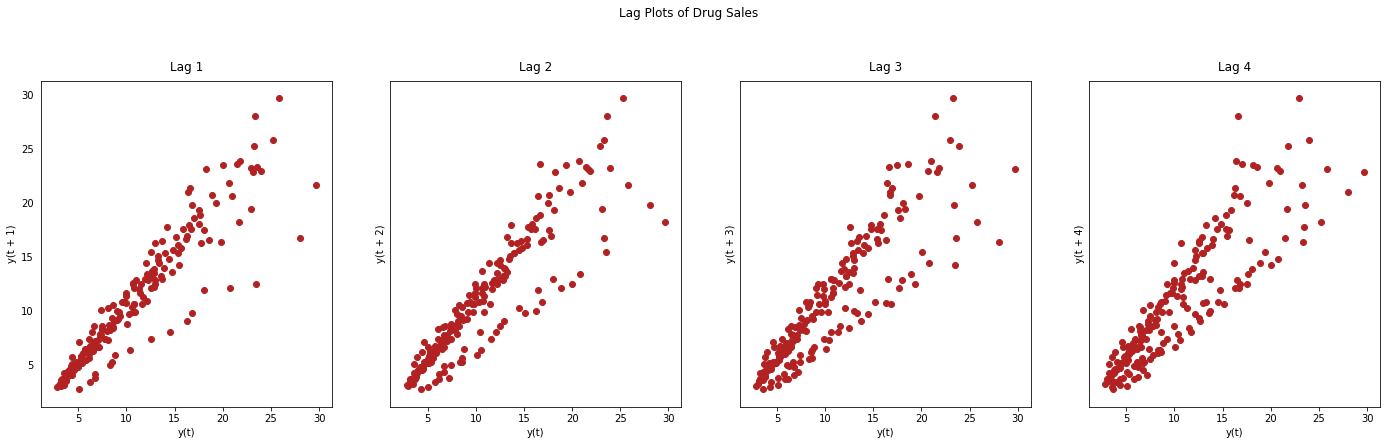
\includegraphics[width=\linewidth]{figures/lag_plot.png}
	\caption{Example of lag plot for our drug sample up to fourth order.}
	\label{fig:lag_plot}
\end{figure}
    
A similar type of quick check that can be done is to directly calculate
the correlation between observation and lag variables. This
can be easily calculated using the \texttt{corr()} function
on the \texttt{DataFrame} of the dataset.

\begin{ipython}
from pandas import concat

dataframe = concat([df['value'].shift(-4), df[4:]['value']], axis=1)
dataframe.columns = ['t-4', 't']
result = dataframe.corr()
print(result)
\end{ipython}
\begin{ioutput}
          t-4         t
t-4  1.000000  0.878839
t    0.878839  1.000000
\end{ioutput}

This is a good confirmation of Fig.~\ref{fig:lag_plot} since the result 
shows a strong
positive correlation (0.88) between the observation and the lag-4 value.

\subsubsection{Autocorrelation Plots}
\label{autocorrelation-plots}

The autocorrelation is comprised of both the direct correlation and indirect correlations. These indirect correlations are a linear function of the correlation of the observation, with lags at intermediate time steps.

A plot of the autocorrelation of a time series as a function of the lag is called the \emph{AutoCorrelation Function} (ACF), sometimes it is also called a correlogram.

In order to plot the autocorrelation coefficient for each lag variable, \texttt{pandas} provides again built-in plot function called \texttt{autocorrelation\_plot()}. The \texttt{statsmodels} library also provides a version of the plot with \texttt{plot\_acf()} function.

The plot provides the lag number along the \(x\)-axis and the correlation coefficient value on the \(y\)-axis. The plot also includes solid and dashed lines that indicate the 95\% and 99\% confidence interval for the correlation values. Correlation values above these lines are more significant than those below the line, providing a threshold or cutoff for selecting more relevant lag values.

In \texttt{statsmodels} is also available the function \texttt{acf} which returns a list with the autocorrelation values.
%\begin{codebox}[breakable, size=fbox, boxrule=1pt, pad at break*=1mm,colback=cellbackground, colframe=cellborder]
%\begin{Verbatim}[commandchars=\\\{\}]
%\PY{k+kn}{from} \PY{n+nn}{pandas}\PY{n+nn}{.}\PY{n+nn}{plotting} \PY{k}{import} \PY{n}{autocorrelation\PYZus{}plot}
%
%\PY{n}{autocorrelation\PYZus{}plot}\PY{p}{(}\PY{n}{df}\PY{p}{[}\PY{l+s+s1}{\PYZsq{}}\PY{l+s+s1}{value}\PY{l+s+s1}{\PYZsq{}}\PY{p}{]}\PY{p}{)}
%\end{Verbatim}
%\end{codebox}
%
%\begin{figure}[htb]
%	\centering
%	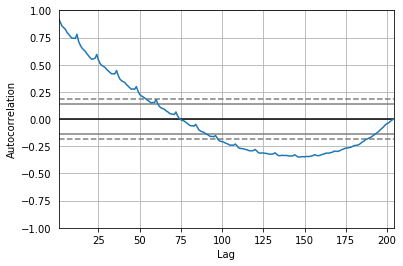
\includegraphics[width=0.7\linewidth]{figures/acf_plot.png}
%	\caption{Example of first and second differencing of the non-stationary time series shown in Fig.~\ref{fig:stationary_non_stationary} (right).}
%	\label{fig:acf}
%\end{figure}

\begin{ipython}
from statsmodels.graphics.tsaplots import plot_acf
from statsmodels.tsa.stattools import acf

plot_acf(df['value'], lags=200)
plt.show()
print (acf(df.value, nlags=20))
\end{ipython}
\begin{ioutput}
[1.        0.92056815 0.88782519 0.85385862 0.84052841 0.82523769
0.79629658 0.77950157 0.75953251 0.74337588 0.74521347 0.74134847
0.78031252 0.71424686 0.68014097 0.65401657 0.63791893 0.62349882
0.60171747 0.58230335 0.5638103 ]
\end{ioutput}
    
\begin{figure}[htb]
	\centering
	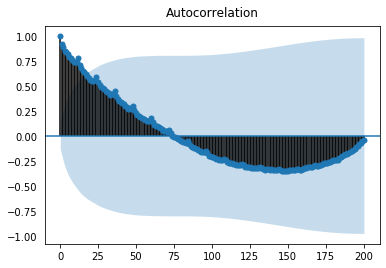
\includegraphics[width=0.7\linewidth]{figures/acf_plot2.png}
	\caption{Example of first and second differencing of the non-stationary time series shown in Fig.~\ref{fig:stationary_non_stationary} (right).}
	\label{fig:acf2}
\end{figure}
    
\subsection{Partial Autocorrelation Function}
\label{partial-autocorrelation-function}

Partial Autocorrelation function (PACF) also conveys similar information to ACF but it only deals with the pure correlation of a series and its lag, excluding the correlation contributions from the intermediate lags.

The partial autocorrelation of lag-\(k\) of a series is the coefficient of that lag in the autoregression equation of \(Y\). For example, the partial autocorrelation of lag-3 is the coefficient \(\phi_3\) in the autoregressive Equation~\ref{eq:ar}.

The \texttt{statsmodels} library also provides a version of the plot with \texttt{plot\_pacf()} function and an accessor to PACF values, \texttt{pacf()}.

\begin{ipython}
from matplotlib import pyplot
from statsmodels.tsa.stattools import pacf
from statsmodels.graphics.tsaplots import plot_pacf

plot_pacf(df.value.tolist(), lags=50)
pyplot.show()
print (pacf(df.value, nlags=20))	
\end{ipython}
\begin{ioutput}
[ 1.          0.92510297  0.28297106  0.0759758   0.16921494  0.09370324
 -0.06396075  0.0560044   0.01650882  0.00431904  0.17496764  0.08742467
  0.41635623 -0.63684013 -0.15223434  0.10337984 -0.10246178  0.04619914
  0.26331492 -0.06447131 -0.05881505]
\end{ioutput}

\begin{figure}[htb]
	\centering
	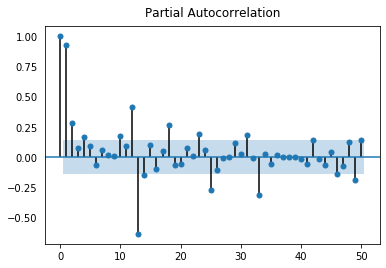
\includegraphics[width=0.7\linewidth]{figures/pacf_plot.png}
	\caption{Example of first and second differencing of the non-stationary time series shown in Fig.~\ref{fig:stationary_non_stationary} (right).}
	\label{fig:pacf}
\end{figure}
    
\subsection{Interpretation or ACF and PACF Plots}
\label{intuition-for-acf-and-pacf-plots}

Plots of the autocorrelation function and the partial autocorrelation function for a time series tell a very different story. 

Consider a time series that was generated by an autoregression (AR) process with a lag-\(k\).

We know that the ACF describes the autocorrelation between an observation and another observation at a prior time step that includes direct and indirect dependence information. This means we would expect the ACF for the AR(\(k\)) time series to be strong to a lag-\(k\) and the 'inertia' of that relationship would carry on to subsequent lag values, trailing off at some point as the effect was weakened.

On the other hand we know that the PACF only describes the direct relationship between an observation and its lag. This would suggest that there would be no correlation for lag values beyond \(k\).

Consider instead a time series that was generated by a moving average (MA)
process with a lag-\(k\).

Remember that the moving average process is an autoregression model of
the time series of residual errors from prior predictions. Another way
to think about the moving average model is that it corrects future
forecasts based on errors made on more recent forecasts.

We would expect the ACF for the MA(\(k\)) process to show a strong
correlation with recent values up to the lag-\(k\), then a sharp decline
to low or no correlation (by definition, this is how the process was
generated).

For the PACF instead, we would expect the plot to show a strong 
relationship to the lag and a trailing off of correlation 
from the lag onwards.

\section{Cointegration}\label{cointegration}

Cointegration tests identify scenarios where two or more non-stationary
time series are integrated together in a way that they cannot deviate
from equilibrium in the long term. They are used to identify the
long-term relationships between two or more sets of variables. The
concept was first introduced by Robert Engle and Clive Granger, in 1987.

Before the introduction of cointegration tests, economists relied on
linear regressions to find the relationship between several time series
processes. However, Granger and Engle argued that linear regression
was an incorrect approach for analyzing time series due to the
possibility of producing spurious correlation.

A spurious correlation occurs when two or more associated variables are
deemed causally related due to either a coincidence or an unknown third
factor. A possible result is a misleading statistical relationship
between several time series variables.

\subsection{Engle-Granger Two-Step Method}
\label{engle-granger-two-step-method}

There are various methods of testing for cointegration. Among them the
Engle-Granger Two-Step method starts by creating residuals based on the
regression of two series and then testing these residuals for
the presence of unit roots (it uses the Augmented Dickey-Fuller test) 
to test for stationarity of the residual series. \emph{If the time
series are cointegrated, the Engle-Granger method, will show the
stationarity of the residuals}.

Let's see an example involving the time series of the number of Google
searches about Milan and Inter football clubs in the last years.
The two series are plotted in Fig.~\ref{fig:cointegrated_series}.

\begin{figure}[htb]
	\centering
	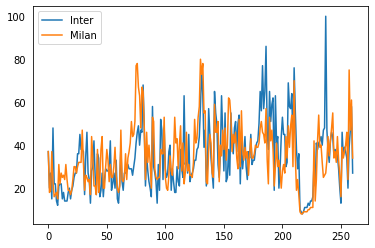
\includegraphics[width=0.7\linewidth]{figures/cointegrated_series.png}
	\caption{Example of first and second differencing of the non-stationary time series shown in Fig.~\ref{fig:stationary_non_stationary} (right).}
	\label{fig:cointegrated_series}
\end{figure}

The following is an implementation of the Engle-Granger test: first regress
one series to the other and find the residuals, then tests this new series
for stationarity. Figure~\ref{fig:residual} shows the residual plot.
   
\begin{codebox}[breakable, size=fbox, boxrule=1pt, pad at break*=1mm,colback=cellbackground, colframe=cellborder]
\begin{Verbatim}[commandchars=\\\{\}]
\PY{k+kn}{import} \PY{n+nn}{statsmodels}\PY{n+nn}{.}\PY{n+nn}{api} \PY{k}{as} \PY{n+nn}{sm}
\PY{k+kn}{from} \PY{n+nn}{statsmodels}\PY{n+nn}{.}\PY{n+nn}{tsa}\PY{n+nn}{.}\PY{n+nn}{stattools} \PY{k}{import} \PY{n}{adfuller}

\PY{n}{ls} \PY{o}{=} \PY{n}{sm}\PY{o}{.}\PY{n}{OLS}\PY{p}{(}\PY{n}{df}\PY{p}{[}\PY{l+s+s1}{\PYZsq{}}\PY{l+s+s1}{inter}\PY{l+s+s1}{\PYZsq{}}\PY{p}{]}\PY{p}{,} \PY{n}{df}\PY{p}{[}\PY{l+s+s1}{\PYZsq{}}\PY{l+s+s1}{milan}\PY{l+s+s1}{\PYZsq{}}\PY{p}{]}\PY{p}{)}
\PY{n}{res} \PY{o}{=} \PY{n}{ls}\PY{o}{.}\PY{n}{fit}\PY{p}{(}\PY{p}{)}

\PY{n}{r} \PY{o}{=} \PY{n}{adfuller}\PY{p}{(}\PY{n}{res}\PY{o}{.}\PY{n}{resid}\PY{p}{)}
\PY{n+nb}{print} \PY{p}{(}\PY{l+s+s2}{\PYZdq{}}\PY{l+s+s2}{test statistic: }\PY{l+s+si}{\PYZob{}\PYZcb{}}\PY{l+s+s2}{\PYZdq{}}\PY{o}{.}\PY{n}{format}\PY{p}{(}\PY{n}{r}\PY{p}{[}\PY{l+m+mi}{0}\PY{p}{]}\PY{p}{)}\PY{p}{)}
\PY{n+nb}{print} \PY{p}{(}\PY{l+s+s2}{\PYZdq{}}\PY{l+s+s2}{p\PYZhy{}value: }\PY{l+s+si}{\PYZob{}\PYZcb{}}\PY{l+s+s2}{\PYZdq{}}\PY{o}{.}\PY{n}{format}\PY{p}{(}\PY{n}{r}\PY{p}{[}\PY{l+m+mi}{1}\PY{p}{]}\PY{p}{)}\PY{p}{)}
\PY{n+nb}{print} \PY{p}{(}\PY{l+s+s2}{\PYZdq{}}\PY{l+s+s2}{alpha 5}\PY{l+s+s2}{\PYZpc{}}\PY{l+s+s2}{ (}\PY{l+s+si}{\PYZob{}\PYZcb{}}\PY{l+s+s2}{)}\PY{l+s+s2}{\PYZdq{}}\PY{o}{.}\PY{n}{format}\PY{p}{(}\PY{n}{r}\PY{p}{[}\PY{l+m+mi}{4}\PY{p}{]}\PY{p}{[}\PY{l+s+s1}{\PYZsq{}}\PY{l+s+s1}{5}\PY{l+s+s1}{\PYZpc{}}\PY{l+s+s1}{\PYZsq{}}\PY{p}{]}\PY{p}{)}\PY{p}{)}

test statistic: -6.105445934885
p-value: 9.609589483491024e-08
alpha 5\% (-2.8728086526320302)
\end{Verbatim}
\end{codebox}

\begin{figure}[htb]
	\centering
	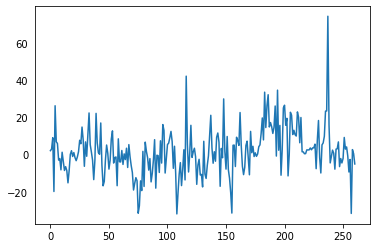
\includegraphics[width=0.7\linewidth]{figures/residual_plot.png}
	\caption{Example of first and second differencing of the non-stationary time series shown in Fig.~\ref{fig:stationary_non_stationary} (right).}
	\label{fig:residual}
\end{figure}
    
The resulting p-value indicates that the residual time series is
stationary so the two initial series are cointegrated.

\section{Granger Causality}\label{granger-causality}

Granger causality test is used to determine if one time series could be
useful to forecast another. It is based on the idea that if \(X\)
Granger-causes \(Y\), then the forecast of \(Y\) based on previous
values of \(Y\) \textbf{and} the previous values of \(X\) should 
outperform the
forecast of \(Y\) based on previous values of \(Y\) alone.

So, understand that Granger causality should not be used to test if a
lag of \(Y\) causes \(Y\). Instead, it is generally used on \emph{exogenous}
(not \(Y\) lag but external) variables only.

A nice implementation of this test is available in the
\texttt{statsmodel} module. It accepts a 2D array with 2 columns as the
main argument. The values are in the first column ($Y$) and the predictor
($X$) is in the second column. The second argument, \texttt{maxlag},
says how many lags of \(Y\) should be included in the test.

The null hypothesis is: the series in the second column, does not
Granger-cause the series in the first. If the p-values are less than a
significance level then you can reject the null hypothesis and conclude
that the said lags of \(X\) are indeed useful.

\begin{codebox}[breakable, size=fbox, boxrule=1pt, pad at break*=1mm,colback=cellbackground, colframe=cellborder]
\begin{Verbatim}[commandchars=\\\{\}]
\PY{k+kn}{from} \PY{n+nn}{statsmodels}\PY{n+nn}{.}\PY{n+nn}{tsa}\PY{n+nn}{.}\PY{n+nn}{stattools} \PY{k}{import} \PY{n}{grangercausalitytests}
\PY{k+kn}{import} \PY{n+nn}{numpy} \PY{k}{as} \PY{n+nn}{np}

\PY{n}{gc\PYZus{}res} \PY{o}{=} \PY{n}{grangercausalitytests}\PY{p}{(}\PY{n}{np}\PY{o}{.}\PY{n}{array}\PY{p}{(}\PY{n}{df}\PY{p}{[}\PY{p}{[}\PY{l+s+s1}{\PYZsq{}}\PY{l+s+s1}{inter}\PY{l+s+s1}{\PYZsq{}}\PY{p}{,}\PY{l+s+s1}{\PYZsq{}}\PY{l+s+s1}{milan}\PY{l+s+s1}{\PYZsq{}}\PY{p}{]}\PY{p}{]}\PY{p}{)}\PY{p}{,} \PY{l+m+mi}{4}\PY{p}{)}

Granger Causality
number of lags (no zero) 1
ssr based F test:         F=5.5471  , p=0.0193  , df\_denom=257, df\_num=1
ssr based chi2 test:   chi2=5.6119  , p=0.0178  , df=1
likelihood ratio test: chi2=5.5522  , p=0.0185  , df=1
parameter F test:         F=5.5471  , p=0.0193  , df\_denom=257, df\_num=1

Granger Causality
number of lags (no zero) 2
ssr based F test:         F=2.5467  , p=0.0803  , df\_denom=254, df\_num=2
ssr based chi2 test:   chi2=5.1938  , p=0.0745  , df=2
likelihood ratio test: chi2=5.1424  , p=0.0764  , df=2
parameter F test:         F=2.5467  , p=0.0803  , df\_denom=254, df\_num=2

Granger Causality
number of lags (no zero) 3
ssr based F test:         F=1.6183  , p=0.1856  , df\_denom=251, df\_num=3
ssr based chi2 test:   chi2=4.9901  , p=0.1725  , df=3
likelihood ratio test: chi2=4.9425  , p=0.1761  , df=3
parameter F test:         F=1.6183  , p=0.1856  , df\_denom=251, df\_num=3

Granger Causality
number of lags (no zero) 4
ssr based F test:         F=2.0213  , p=0.0920  , df\_denom=248, df\_num=4
ssr based chi2 test:   chi2=8.3788  , p=0.0786  , df=4
likelihood ratio test: chi2=8.2451  , p=0.0830  , df=4
parameter F test:         F=2.0213  , p=0.0920  , df\_denom=248, df\_num=4
\end{Verbatim}
\end{codebox}

\begin{thebibliography}{9}
\bibitem{bib:dictionary_of_stats} B. S. Everitt, A. Skrondal, \emph{The Cambridge
	Dictionary of Statistics}, Cambridge University Press, 2010. 
\bibitem{bib:cartoon} L. Gonick, \emph{The Cartoon Guide to Statistics}, HarperPerennial, 1993
\bibitem{bib:t_dist} Meier et. al, \emph{Applied Statistics for Public and Nonprofit Administration}, Cengage Learning, 1999
\bibitem{bib:t_dist2} \href{}{\emph{https://simon.cs.vt.edu/SoSci/converted/T-Dist/}}, 2016, [Online]
\end{thebibliography}
